\chapter{Event and candidate selection}
\label{chap:prod:sel}

The decay modes chosen for this analysis,
\DzToKpi, \DpToKpipi, \DspTophipi\ with \phiToKK, and \DstToDzpi\ with 
\DzToKpi, including their charge conjugates, are the amongst the most probable 
fully charged, hadronic final states for each charm meson.
The advantage of reconstructing such final states is that it allows the 
invariant mass of the charm hadrons to be computed unambiguously, so that a 
yield determination can be performed by modelling the peaking signal structure 
in the mass distribution via fits.
These fits will be discussed in detail in \cref{chap:prod:fitting}, but it is 
worth noting at this point that such fits are simpler if the data is `clean', 
that is if the fraction of charm meson signal in the data is high.
It is then advantageous to optimise the selection of the data to reduce 
backgrounds, whilst retaining as much signal as possible to maximise the 
statistical precision of the measurement.

The selection of fully charged, hadronic decay modes of charm mesons has 
already been performed by many other analyses at \lhcb\footnotemark\ and their 
selections share several common features.
\footnotetext{%
  Representative examples include selections of 
  \decay{\PDzero}{\PKmp\Ppipm}~\cite{Aaij:2012nva}, 
  \decay{\PDp}{\PKminus\PKplus\Ppiplus}~\cite{Aaij:2011cw}, and 
  \DspTophipi~\cite{Aaij:2012cy} decays.
}
The first of these features is a requirement on the minimum charm candidate 
\pT, as there are many soft particles produced directly in the proton-proton 
collision.
The second is to ask that the charm candidate vertex is significantly displaced 
from the \ac{PV}, exploiting the long lifetimes of charm hadrons in the 
laboratory frame.
Finally, it is required that the \ipchisq\ of the charm meson, a measure of the 
\acf{IP} significance, does not exceed a certain value.
This suppresses the background of charm candidates whose three-momentum does 
not point back to the \ac{PV}.
Each of these three features are powerful discriminators between signal and 
background.

For this measurement of prompt charm production it is preferable not to make 
\pT\ requirements on the charm candidate as the \pT\ range available for 
differential measurements would be restricted.
Nor is it desirable to make \ipchisq\ cuts, as the \ipchisq\ distribution is 
used for prompt-secondary discrimination.
The selection used is then informed by previous \lhcb\ studies of fully 
charged, hadronic charm decays, but with modifications to improve the utility 
for the measurement in hand.
The selection variables that are useful for discriminating between signal and 
background, in addition to those already discussed, are given and described 
below.
The `parent' is the charm hadron \PHc, and the `children' are the charged 
hadrons in the final state.

The child tracks are firstly selected based on the quality of the track fit, 
the track fit \chisq\ per degree of freedom.
For fake~(ghost) tracks, the \chisq\ is higher on average.
Child \ptot\ and \Eta\ are required to be in the range in which calibration 
samples are available for \ac{PID} efficiency measurements (described in more 
detail in \cref{chap:prod:effs:pid}).
The track \pT\ is required to be above some minimum to reduce the background 
from random soft tracks originating from the \ac{PV}, and similarly for the 
track \ipchisq, which will be high on average for tracks produced from a 
displaced, secondary vertex.
Finally, \ac{PID} requirements are made on the tracks to reduce 
misidentification backgrounds, particularly to suppress the large fraction of 
pions in the event when a kaon candidate is required.

The combination of tracks used to form an \PHc\ candidate is required to have a 
maximum pairwise \ac{DOCA} less than some value.
If a vertex can be fitted using the combination, the \chisq\ of the fit should 
be low, indicating a good compatibility with the physical vertex hypothesis.
For long-lived charm hadrons, the vertex can be significantly displaced from 
the \ac{PV}, and making a minimum requirement on the displacement suppresses 
much combinatorial background.
The momentum vector of the \PHc\ candidate should have the same direction as 
that of the vector that points from the \ac{PV} to the decay vertex, and the 
angle between these two vectors, the \ac{DIRA}, is required to be less than 
some value.
Finally, the reconstructed mass of the parent vertex must be near the nominal 
mass of the hadron under study.
A suitably large window must be used on order to be able to accurately model 
the combinatorial background shape in the mass fits.

The numerical requirements made on the discriminatory quantities were not tuned 
to optimise any specific figure of merit.
Instead, the values were chosen based on those used in previous charm analyses, 
generally being loosened to account for the higher rate available to charm 
triggers during the early measurements period, and the desire to have as high 
an efficiency as possible in the low \pT\ regions of the measurement.

As this analysis uses the Turbo stream, the only selection is that defined 
using `online' quantities computed in the trigger.
The same quantities are used `offline', with no further reconstruction being 
performed.
The description of the selection is split in two: the `online' part, which is 
the selection defined in the trigger and cannot be tuned once the data have 
been taken, and the `offline' selection, which is any selection made after the 
online.

\section{Online selection and reconstruction}
\label{chap:prod:sel:online}

The different purposes and hierarchy of the different stages of the \lhcb\ 
trigger are described in \cref{chap:intro:lhcb:trigger}.
For this analysis, at \lzero\ bunch-bunch crossings are accepted randomly by 
the \nobias\ trigger.
The rate at which the \nobias\ trigger accepts events is programmed into the 
hardware controller manually, with the exact rate depending on the number of 
colliding bunches at \lhcb.
The rates were tuned throughout the early measurements period so as to keep the 
detector `dead time' to a minimum.\footnotemark\
The \lzero\ rate is given for each fill in 
\cref{tab:prod:sel:online:l0_nobias_rateeff}.
\footnotetext{%
  The detector dead time is the period during which triggers by the \lzero\ are 
  `lost' due to the read-out buffer being full.
  The buffer is able to hold 16 events, each of which takes 40 \ac{LHC} clock 
  cycles, of \SI{25}{\nano\second} each, to be sent to the \hlt.
  Dead time can then occur if several triggers occur too close to one 
  another~\cite{Schmelling:1998qta}.
}

In \hltone, the following sequence is performed for events passing \lzero:
\begin{enumerate}
  \item The full offline charged particle (track) reconstruction is run for 
    hits inside the \velo\ sub-detector;
  \item The full offline \ac{PV} reconstruction is run, using as input only the 
    \velo\ tracks reconstructed in the previous step; and
  \item The reconstruction of `long' tracks, by first extrapolating \velo\ 
    tracks into the \ttracker\ and then, if at least two matching hits are 
    found in the \ttracker, extrapolating through the magnetic field.
    To decrease the time taken to assess all combinatorial combinations of 
    \velo+\ttracker\ tracks with hits in the \itracker\ and \otracker, only 
    hits within a search window assuming a \pT\ of at least \SI{800}{\MeVc} are 
    considered.
\end{enumerate}
Requiring all child tracks from a vertex to have $\pT > \SI{800}{\MeVc}$ would 
be inefficient for low \pT\ charm hadrons, and so the full decay is not 
reconstructed in \hltone.
Instead, the presence of a single, good quality track is required, which is 
consistent with having originated from a heavy flavour decay by having a large 
\ipchisq.
The full set of selection requirements is given in 
\cref{tab:prod:sel:online:hlt1_selection}.

\hlttwo\ performs the full, offline-quality event reconstruction on events 
passing \hltone.
One \hlttwo\ line is defined per charm decay topology, corresponding to: one 
line for \DzToKpi; one line for the charged three-body decays, specifically 
\DpToKpipi\ and \DspToKKpi; and one line for \DstToDzpi.
In the \PDzero, \PDplus, and \PDsplus lines, candidates are made by combining 
long tracks whose particle hypotheses are consistent with the final state under 
consideration.
In the \PDstarp\ line, \PDzero\ candidates passing the \PDzero\ \hlttwo\ line 
are combined with pion candidates, referred to here as `soft pions', 
\Ppiplussoft.
There are three stages to the particle combination: when cuts are applied to 
the input tracks; when cuts are applied to the four-vector sum of these tracks; 
and when cuts are applied to the fitted vertex.
To save computing resources, the combination does not proceed past a failing 
step, and combinations where the vertex fit fails to converge are discarded, 
although the likelihood of a failing vertex fit is suppressed by making 
\ac{DOCA} requirements beforehand.
An event is saved for offline analysis if at least one \hlttwo\ line `fired', 
that is if a charm candidate is made that passes all cuts.
The \DzToKpi, \DTohhh, and \DstToDzpi\ requirements are given in 
\cref{tab:prod:sel:online:hlt2_dztokpi_selection,tab:prod:sel:online:hlt2_dtohhh_selection,tab:prod:sel:online:hlt2_dsttodzpi_selection}.
Distributions of the invariant masses of the charm candidates after the trigger 
selection are given in 
\cref{fig:prod:sel:D0ToKpi:online,fig:prod:sel:DpToKpipi:online,fig:prod:sel:DsToKKpi:online,fig:prod:sel:DstToD0pi_D0ToKpi:online}.

\begin{table}
  \caption{%
    List of fills used in the analysis, along with the integrated luminosity 
    \intlumi, the \lzero\ \nobias\ rate, and the corresponding effective 
    \lzero\ efficiency (``eff.'') for each fill.
  }
  \label{tab:prod:sel:online:l0_nobias_rateeff}
  \centering
  \begin{tabular}{lS[table-figures-uncertainty=1]cS[table-format=2.2]}
  \toprule
  Fill number & {\intlumi (\si{\per\nb})} & \lzero\ \nobias\ rate (\si{\kilo\hertz}) & {\lzero\ \nobias\ eff. (\si{\percent})} \\
  \midrule
  3976        & 628 \pm 24                & 250                                      & 20.58                                   \\
  3981        & 1101 \pm 43               & 300                                      & 10.84                                   \\
  3988        & 931 \pm 36                & 300                                      & 10.84                                   \\
  3992        & 1310 \pm 51               & 350                                      & 7.84                                    \\
  3996        & 999 \pm 39                & 350                                      & 7.84                                    \\
  \bottomrule
\end{tabular}

\end{table}

\begin{table}
  \caption{%
    Requirements made on the track that fires the \hltone\ trigger line.
  }
  \label{tab:prod:sel:online:hlt1_selection}
  \centering
  \begin{tabular}{lcc}
  \toprule
  Particle                   & Variable     & Cut value          \\
  \midrule
  \multirow{5}{*}{Any track} & \pT          & $> \SI{800}{\MeV}$ \\
                             & \ptot        & $> \SI{3}{\GeV}$   \\
                             & Track \chisq & $< 3$              \\
                             & \ipchisq     & $> 10$             \\
                             & \velo\ hits  & $> 9$              \\
  \bottomrule
\end{tabular}

\end{table}

\begin{table}
  \caption{%
    Requirements made in the \hlttwo\ \DzToKpi\ selection.
    The track \chisq\ criterion is applied in the reconstruction and listed 
    here for completeness.
  }
  \label{tab:prod:sel:online:hlt2_dztokpi_selection}
  \centering
  \begin{tabular}{lccc}
  \toprule
  Particle                        & Variable                   &
  Cut value                      \\
  \midrule
  \multirow{4}{*}{\Ppipm, \PKpm}  & \pT                        & $> \SI{250}{\MeV}$                      \\
                                  & \ptot                      & $\ptot > \SI{2}{\GeV}$                  \\
                                  & Track \chisq               & $< 3$                                   \\
                                  & \ipchisq                   & $> 16$                                  \\
  \midrule
  \Ppipm                          & \dllkpi                    & $< 5$                                   \\
  \midrule
  \PKpm                           & \dllkpi                    & $> 5$                                   \\
  \midrule
  \multirow{5}{*}{\PDzero}        & $m(\PKminus\Ppiplus)$      & $\SI{1784}{\MeV} < m < \SI{1944}{\MeV}$ \\
                                  & \PK to \Ppi DOCA           & $< \SI{0.1}{mm}$                        \\
                                  & Vertex fit \chisq          & $< 10$                                  \\
                                  & Direction angle            & $< \SI{17}{\milli\radian}$              \\
                                  & Vertex displacement \chisq & $> 49$                                  \\
  \bottomrule
\end{tabular}

\end{table}

\begin{table}
  \caption{%
    Requirements made in the \hlttwo\ \DTohhh\ selection.
    The \PDp and \PDsplus candidates are defined according to the three-body 
    mass window after the vertex fit.
    Cuts of the form $x > x_{1},\, x_{2},\, x_{3}$ require that all particles 
    satisfy $x > x_{1}$, at least two satisfy $x > x_{2}$, and at least one 
    satisfies $x > x_{3}$.
    The track \chisq\ criterion is applied in the reconstruction and listed 
    here for completeness.
  }
  \label{tab:prod:sel:online:hlt2_dtohhh_selection}
  \centering
  \begin{tabular}{lccc}
  \toprule
  Particle                          & Variable                   & Cut value                                           \\
  \midrule
  \multirow{4}{*}{\Ppipm, \PKpm}    & \pT                        & $> 200,\, 400,\, \SI{1000}{\MeV}$                   \\
                                    & \ptot                      & $\ptot > \SI{2}{\GeV}$                              \\
                                    & Track \chisq               & $< 3$                                               \\
                                    & \ipchisq                   & $> 4,\, 10,\, 50$                                   \\
  \midrule
  \Ppipm                            & \dllkpi                    & $< 5$                                               \\
  \midrule
  \PKpm                             & \dllkpi                    & $> 5$                                               \\
  \midrule
  \PDplus                           & $m(\Phm\Php\Php)$          & $\SI{1789}{\MeV} < m < \SI{1949}{\MeV}$             \\
  \midrule
  \PDsplus                          & $m(\Phm\Php\Php)$          & $\SI{1889}{\MeV} < m < \SI{2049}{\MeV}$             \\
  \midrule
  \multirow{3}{*}{\PDplus/\PDsplus} & Vertex fit \chisq          & $< 25$                                              \\
                                    & Direction angle            & $< \SI{35}{\milli\radian}$                          \\
                                    & Vertex displacement \chisq & $> 16$ \text{AND} $\tau > \SI{0.150}{\pico\second}$ \\
  \bottomrule
\end{tabular}

\end{table}

\begin{table}
  \caption{%
    Requirements made in the \hlttwo\ \DstToDzpi\ selection.
    The input \PDzero\ candidates are those passing the \PDzero selection 
    defined in \cref{tab:prod:sel:online:hlt2_dztokpi_selection}.
    The track \chisq\ criterion is applied in the reconstruction and listed 
    here for completeness.
  }
  \label{tab:prod:sel:online:hlt2_dsttodzpi_selection}
  \centering
  \begin{tabular}{lccc}
  \toprule
  Particle                  & Variable                 & Cut value                             \\
  \midrule
  \multirow{2}{*}{\Ppipm}   & \pT                      & $> \SI{100}{\MeV}$                    \\
                            & Track \chisq             & $< 3$                                 \\
  \midrule
  \multirow{2}{*}{\PDstarp} & $m(\PDstarp)-m(\PDzero)$ & $\SI{130}{\MeV} < m < \SI{160}{\MeV}$ \\
                            & Vertex fit \chisq        & $< 25$                                \\
  \bottomrule
\end{tabular}

\end{table}

\section{Offline selection}
\label{chap:prod:sel:offline}

To improve the purity of the samples, the pion \ac{PID} requirement is 
tightened to $\dllkpi < 3$.
Furthermore, kinematic requirements are made on all \PDzero, \PDplus, and 
\PDsplus children such that they are within the fiducial region of phase space 
available for \ac{PID} efficiency calibration, specifically ${3 < \ptot < 
  \SI{100}{\GeVc}}$ and ${2 < \Eta < 5}$.
As the three-body samples contain a large fraction of combinatorial background 
even after these additional cuts, the vertex fit \chisq\ and the direction 
angle cuts are tightened to $\chisq < 6$ and $\ac{DIRA} < 
\SI{14}{\milli\radian}$.

To reduce the combinatorial background further in the \DspToKKpi\ data, a 
requirement is made on the kaon pair as
\begin{equation}
  999.46 < m(\PKminus\PKplus) < \SI{1039.46}{\MeVcc}.
  \label{eqn:prod:sel:phi_cut}
\end{equation}
This corresponds to a $\pm\SI{20}{\MeVcc}$ window around the nominal mass of 
the $\phi(1020)$ meson~\cite{PDG2014}, which is referred to here as just 
`\Pphi'.
Around half of all \DspToKKpi\ decays proceed via the 
$\decay{\Pphi}{\PKminus\PKplus}$ channel~\cite{PDG2014}, and the narrow width 
of the \Pphi resonance makes this cut efficient at reducing the fraction of 
combinatorial background in the data, as well as reducing the fraction of $\Ppi 
\to \PK$ mis-identifications.
As the \DspToKKpi sample is then dominated by resonant \DspTophipi, the 
\PDsplus sample is referred as `\DspTophipi'.
The effective reduction of the total number of \PDsplus mesons produced due to 
the \Pphi requirement is treated as part of the branching fraction contribution 
in \cref{eqn:prod:introduction:differential_cross_section}, rather than as part 
of the selection efficiency.
The \DspTophipi\ branching fraction used is that given by the \cleo\ 
collaboration, where the same $\PKm\PKp$ mass window definition is 
used~\cite{Alexander:2008aa}, and hence includes the branching fraction of the 
\phiToKK\ decay.

The charm candidate invariant mass distributions after the full offline 
selection are given in 
\cref{fig:prod:sel:D0ToKpi:offline,fig:prod:sel:DpToKpipi:offline,fig:prod:sel:DsToKKpi:offline,fig:prod:sel:DstToD0pi_D0ToKpi:offline}.
The number of charm candidates before and after the offline requirements are 
given in \cref{tab:prod:sel:candidates}.

\begin{figure}
  \begin{subfigure}[b]{0.5\textwidth}
    \centering
    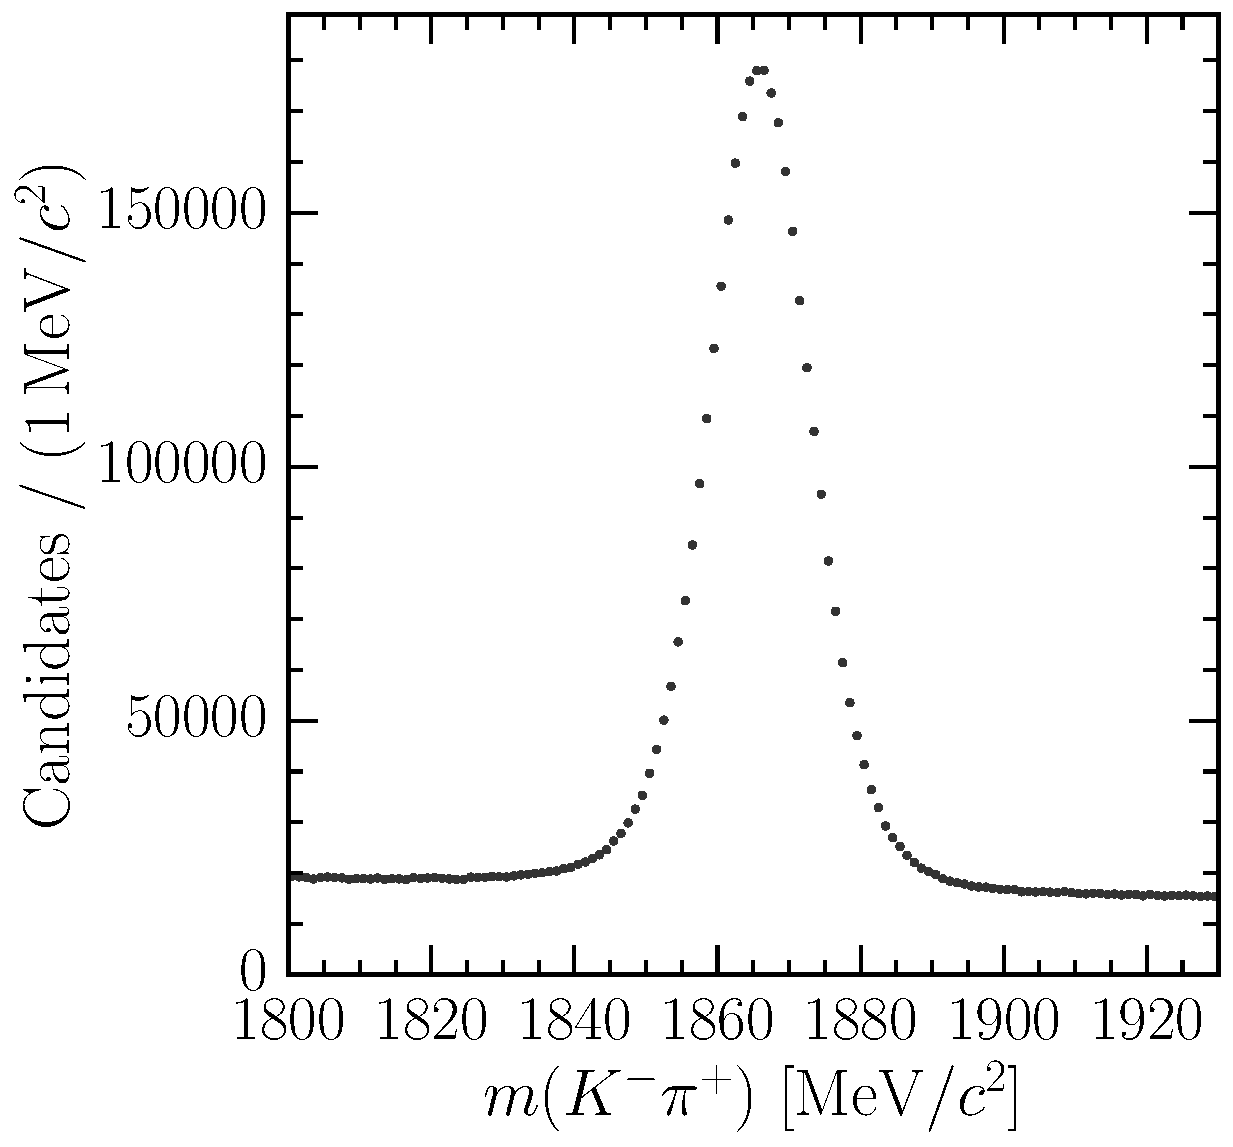
\includegraphics[width=\textwidth]{production/selection/D0ToKpi_mass}
    \caption{Online selected}
    \label{fig:prod:sel:D0ToKpi:online}
  \end{subfigure}
  \begin{subfigure}[b]{0.5\textwidth}
    \centering
    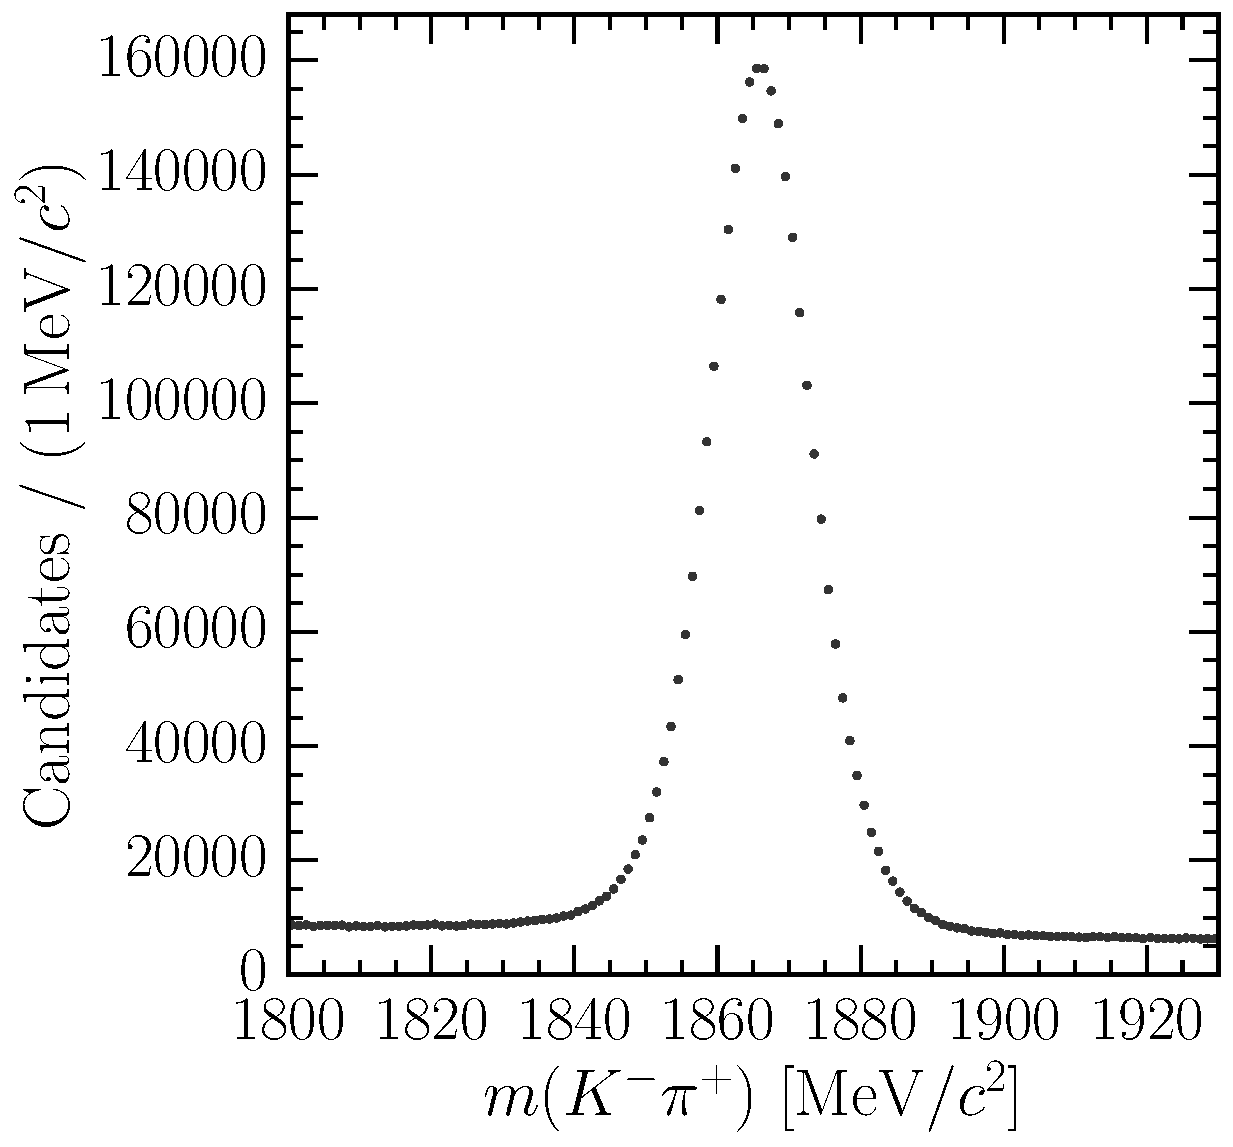
\includegraphics[width=\textwidth]{production/selection/D0ToKpi_mass_offline_selection}
    \caption{Offline selected}
    \label{fig:prod:sel:D0ToKpi:offline}
  \end{subfigure}
  \caption{%
    Mass distributions of \DzToKpi\ candidates after the online (trigger) 
    selection (\subref*{fig:prod:sel:D0ToKpi:online}) and after the offline 
    selection (\subref*{fig:prod:sel:D0ToKpi:offline}).
  }
  \label{fig:prod:sel:D0ToKpi}
\end{figure}

\begin{figure}
  \begin{subfigure}[b]{0.5\textwidth}
    \centering
    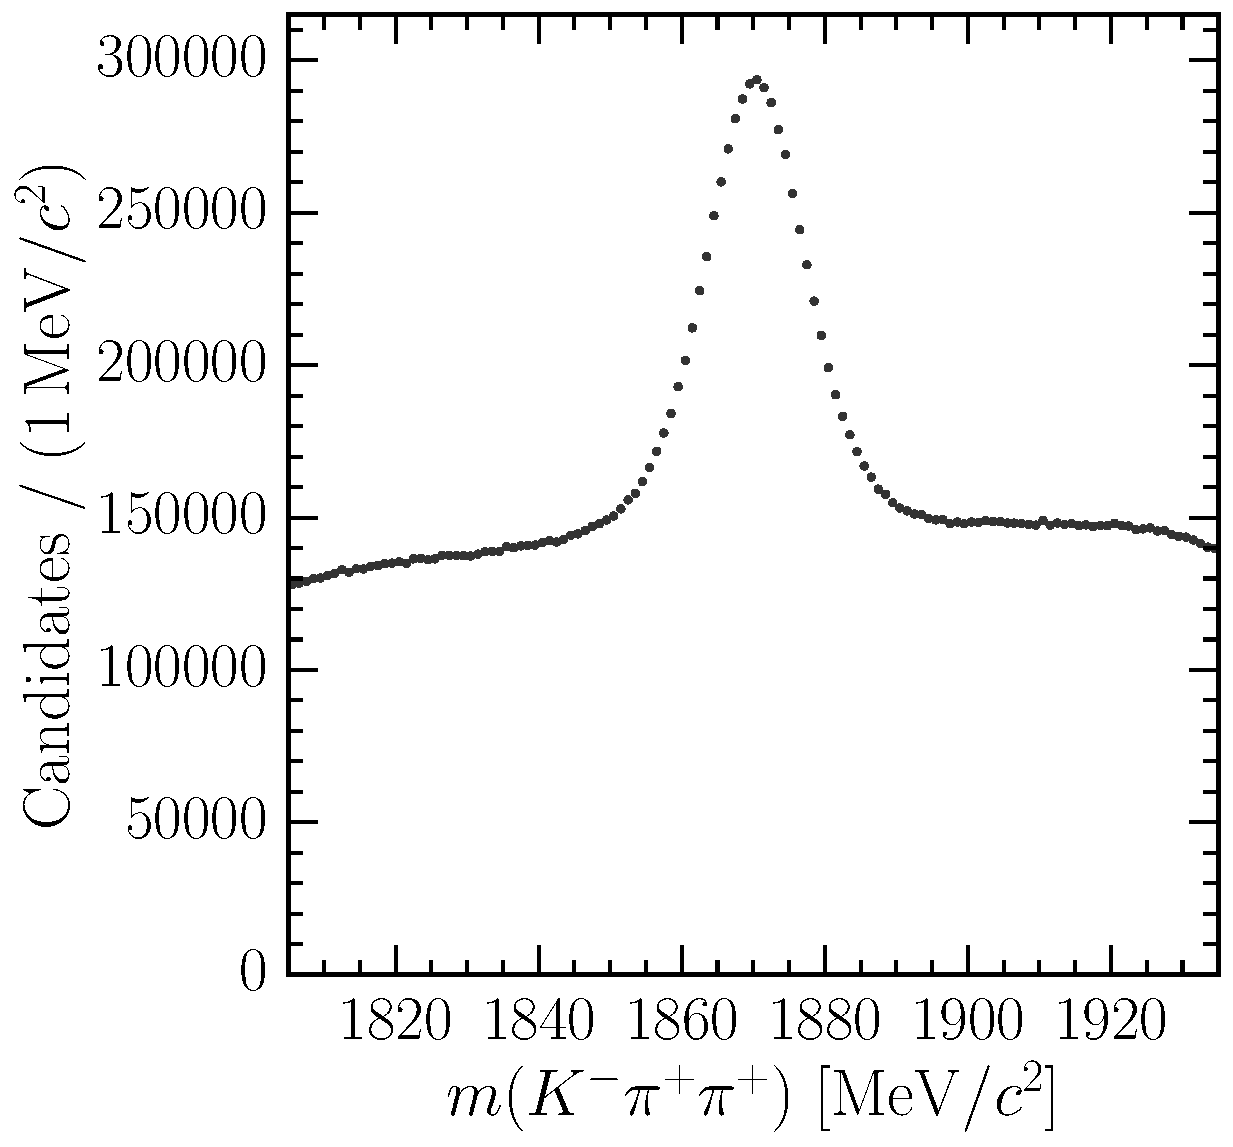
\includegraphics[width=\textwidth]{production/selection/DpToKpipi_mass}
    \caption{Online selected}
    \label{fig:prod:sel:DpToKpipi:online}
  \end{subfigure}
  \begin{subfigure}[b]{0.5\textwidth}
    \centering
    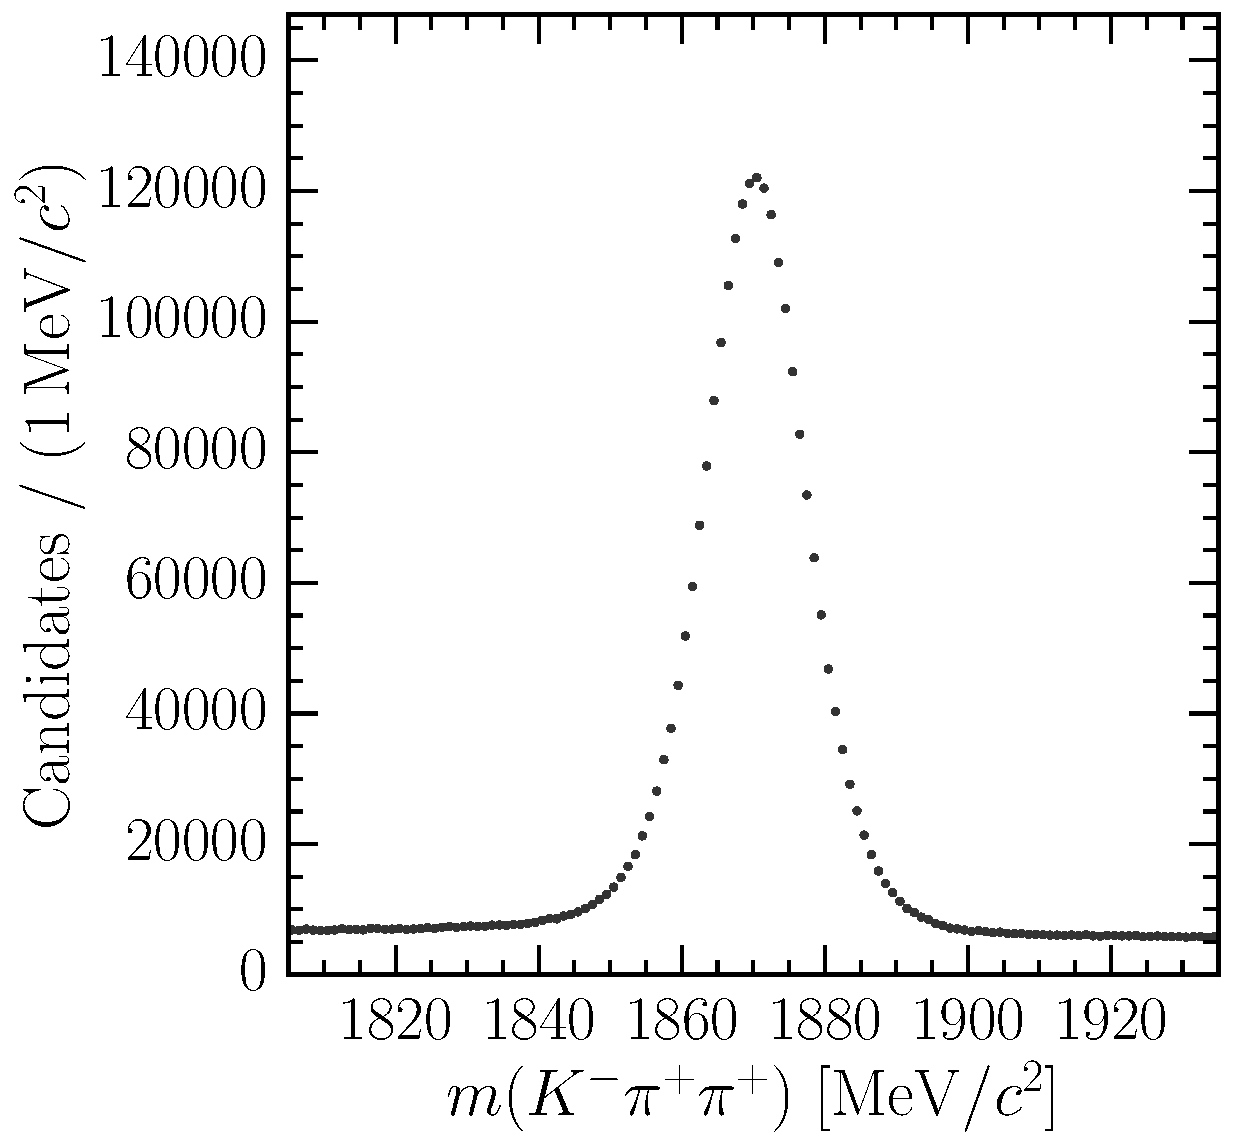
\includegraphics[width=\textwidth]{production/selection/DpToKpipi_mass_offline_selection}
    \caption{Offline selected}
    \label{fig:prod:sel:DpToKpipi:offline}
  \end{subfigure}
  \caption{%
    Mass distributions of \DpToKpipi\ candidates after the online (trigger) 
    selection (\subref*{fig:prod:sel:DpToKpipi:online}) and after the offline 
    selection (\subref*{fig:prod:sel:DpToKpipi:offline}).
  }
  \label{fig:prod:sel:DpToKpipi}
\end{figure}

\begin{figure}
  \begin{subfigure}[b]{0.5\textwidth}
    \centering
    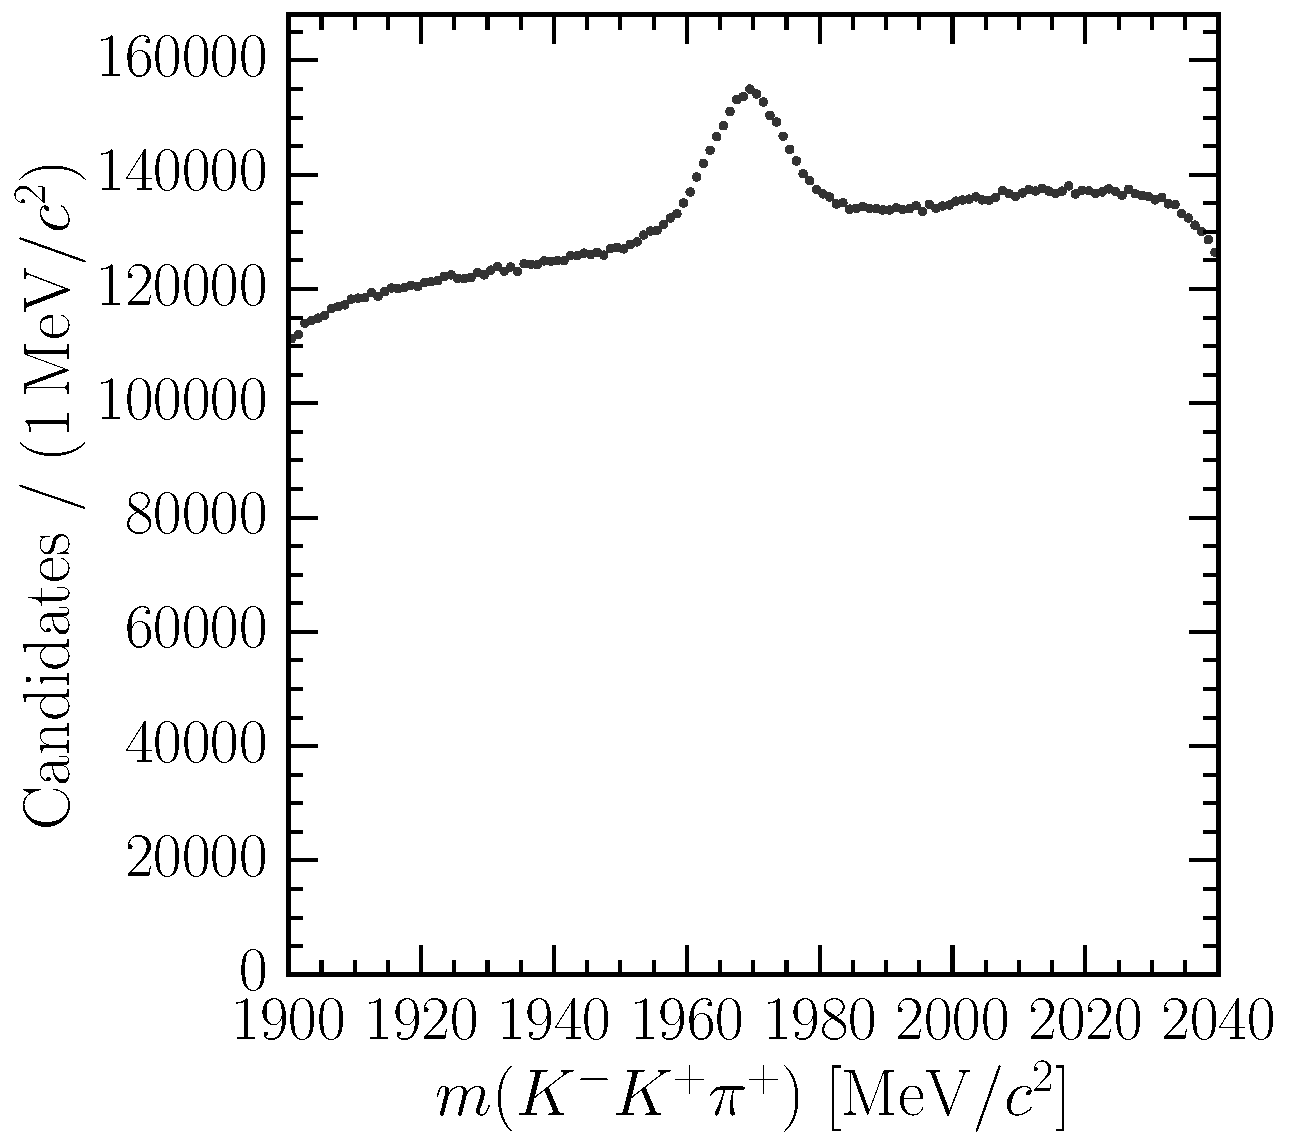
\includegraphics[width=\textwidth]{production/selection/DsToKKpi_mass}
    \caption{Online selected}
    \label{fig:prod:sel:DsToKKpi:online}
  \end{subfigure}
  \begin{subfigure}[b]{0.5\textwidth}
    \centering
    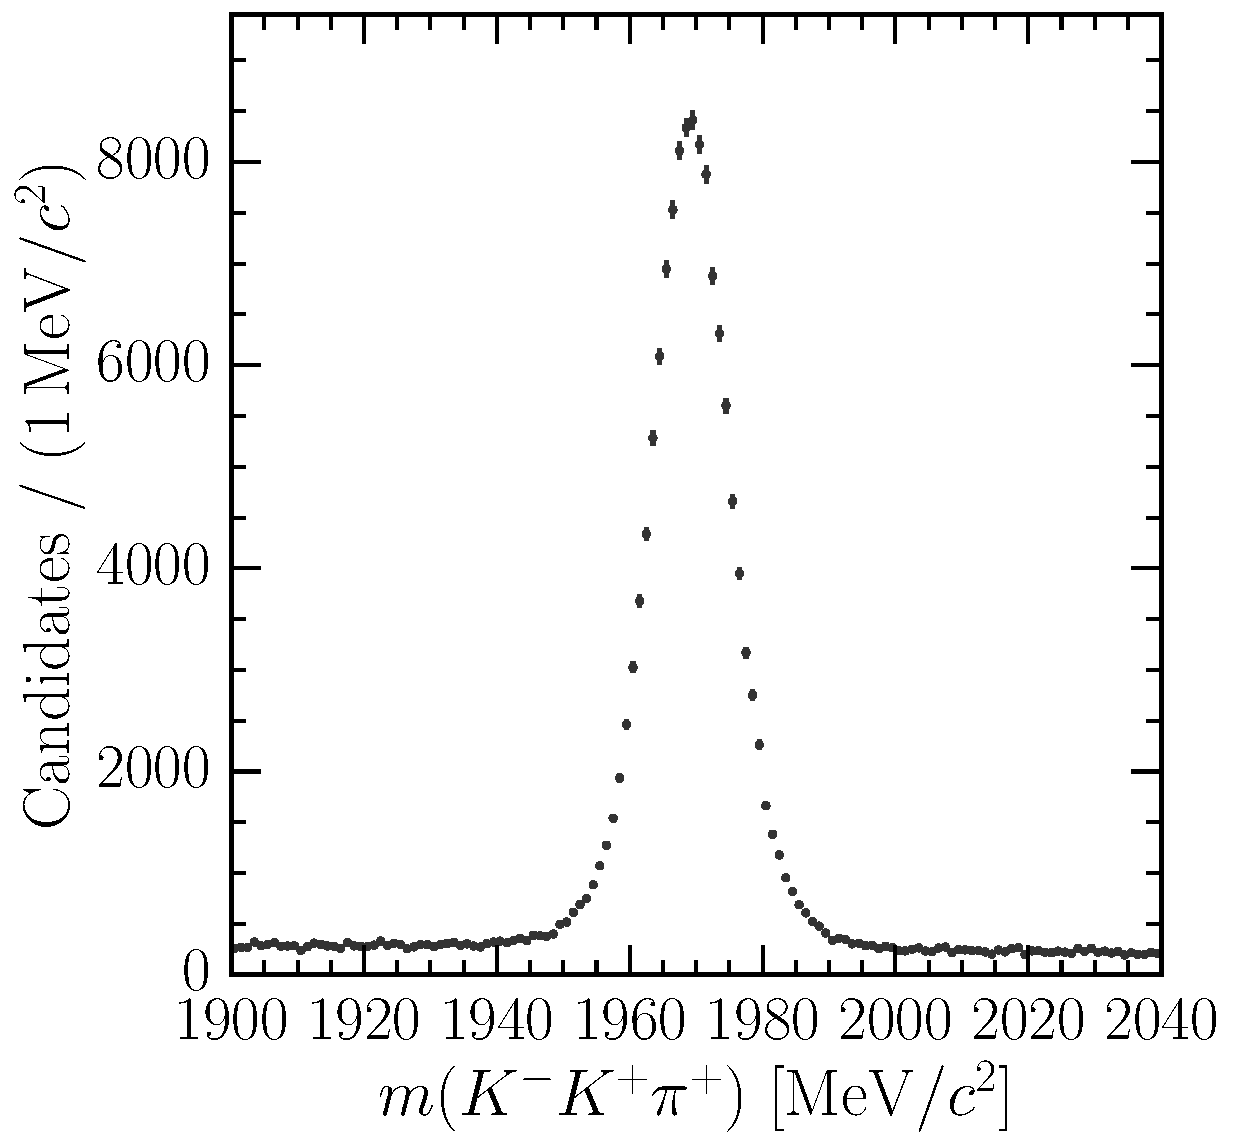
\includegraphics[width=\textwidth]{production/selection/DsToKKpi_mass_offline_selection}
    \caption{Offline selected}
    \label{fig:prod:sel:DsToKKpi:offline}
  \end{subfigure}
  \caption{%
    Mass distributions of \DspToKKpi\ candidates after the online (trigger) 
    selection (\subref*{fig:prod:sel:DsToKKpi:online}) and after the offline 
    selection (\subref*{fig:prod:sel:DsToKKpi:offline}).
    The offline selection includes the requirement that the kaon pair are 
    within a $\pm\SI{20}{\MeVcc}$ window around the nominal $\phi(1020)$ mass.
  }
  \label{fig:prod:sel:DsToKKpi}
\end{figure}

\begin{figure}
  \begin{subfigure}[b]{0.5\textwidth}
    \centering
    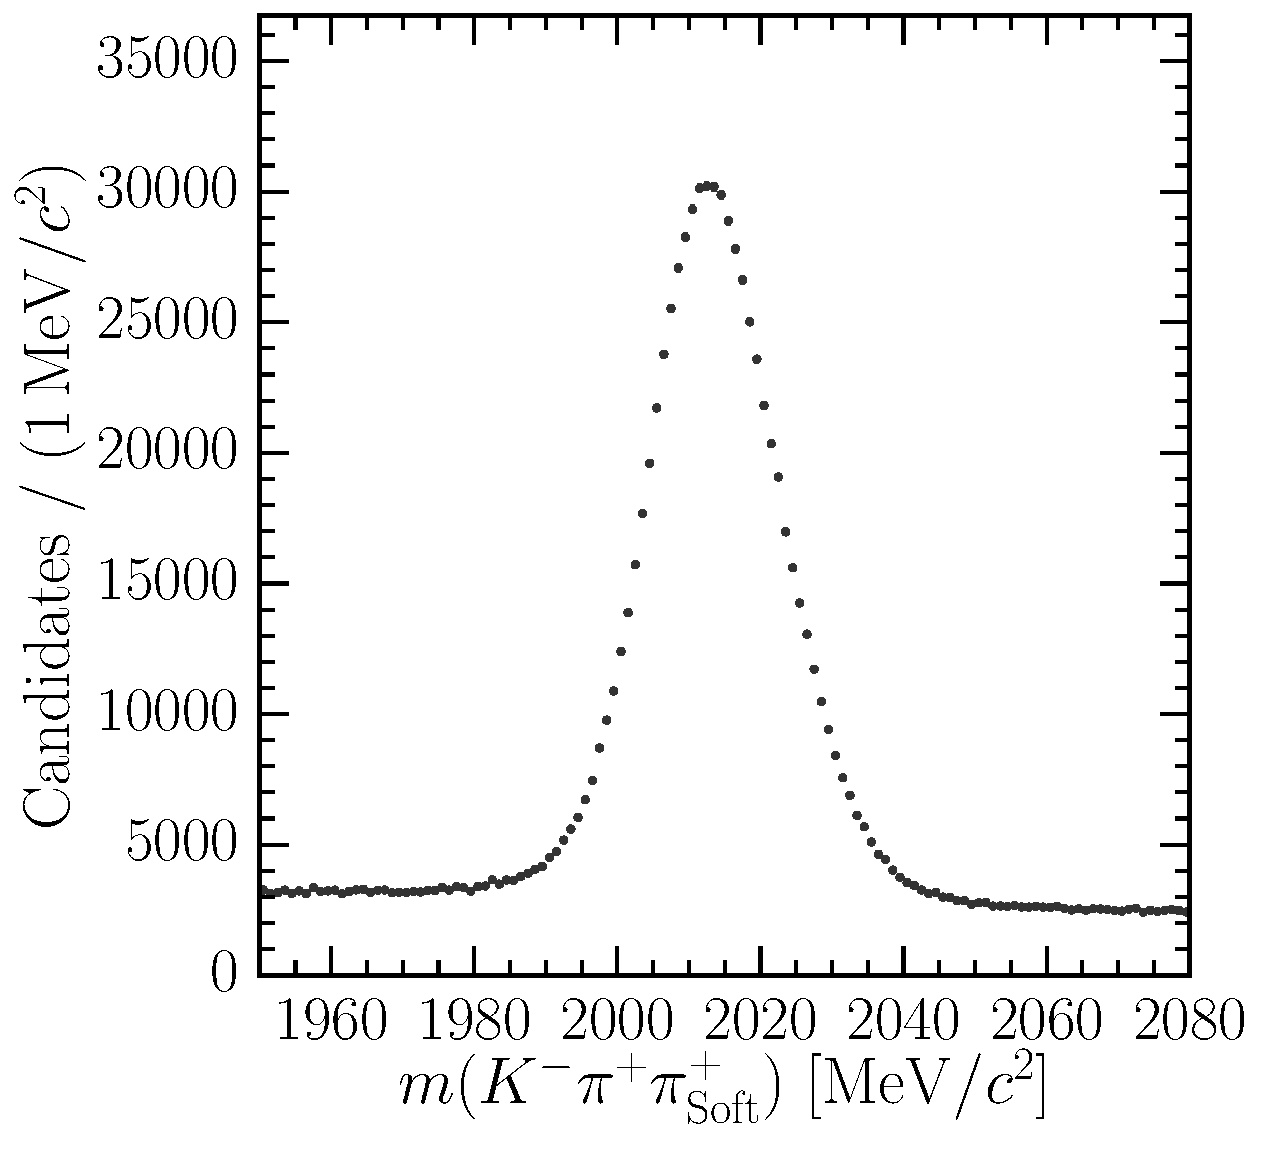
\includegraphics[width=\textwidth]{production/selection/DstToD0pi_D0ToKpi_mass}
    \caption{Online selected}
    \label{fig:prod:sel:DstToD0pi_D0ToKpi:online}
  \end{subfigure}
  \begin{subfigure}[b]{0.5\textwidth}
    \centering
    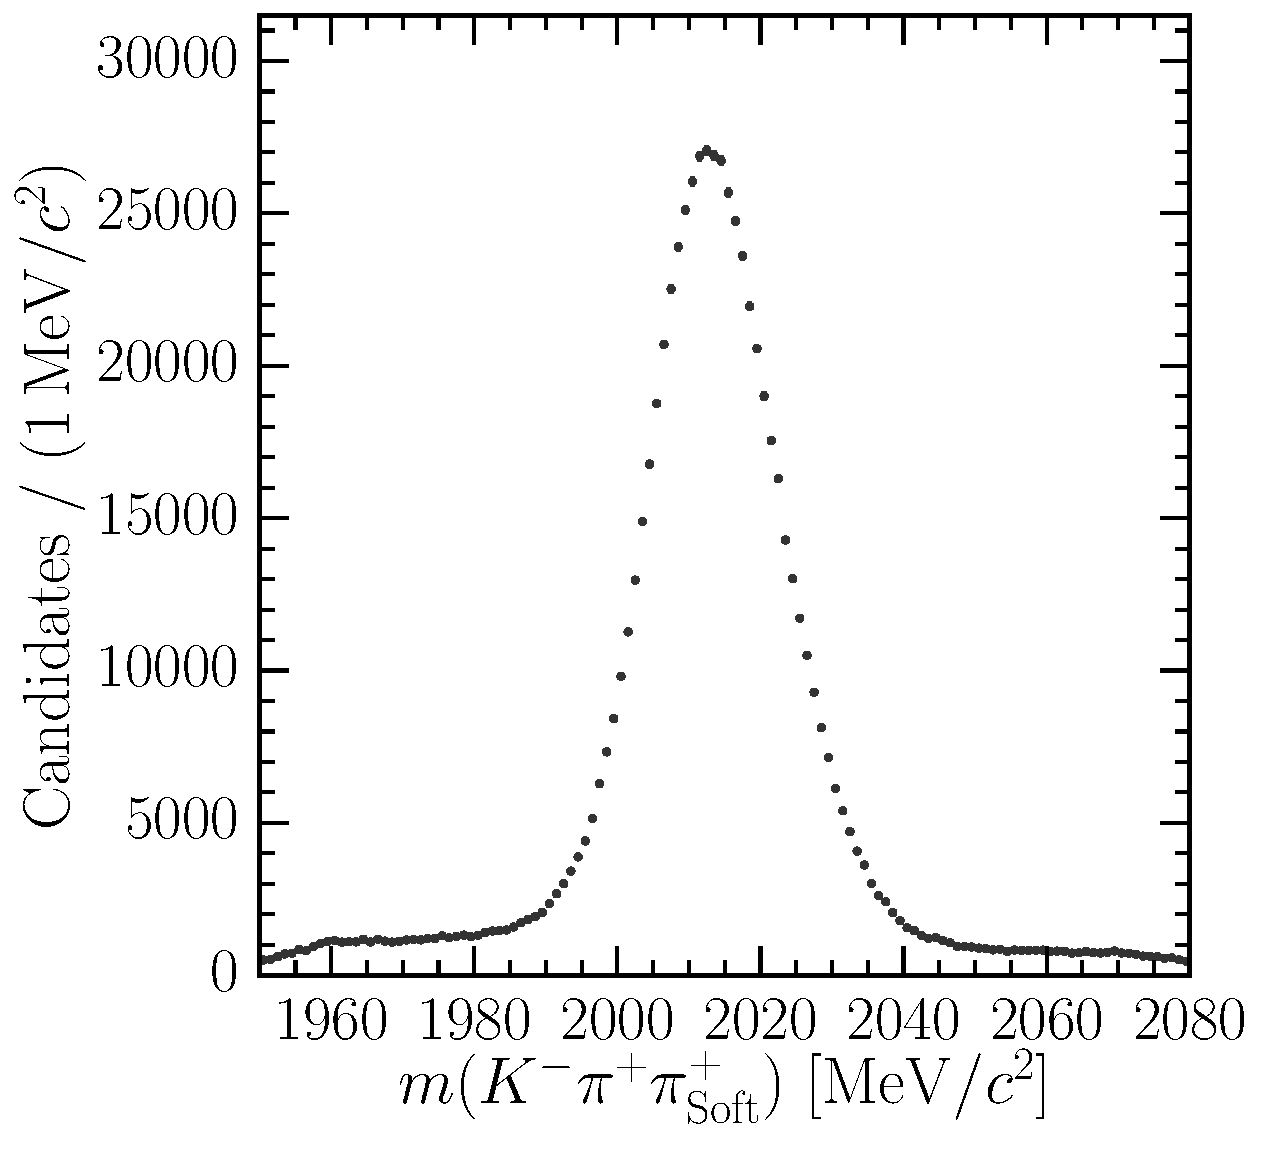
\includegraphics[width=\textwidth]{production/selection/DstToD0pi_D0ToKpi_mass_offline_selection}
    \caption{Offline selected}
    \label{fig:prod:sel:DstToD0pi_D0ToKpi:offline}
  \end{subfigure}
  \caption{%
    Mass distributions of \DstToDzpi\ candidates after the online (trigger) 
    selection (\subref*{fig:prod:sel:DstToD0pi_D0ToKpi:online}) and after the 
    offline selection (\subref*{fig:prod:sel:DstToD0pi_D0ToKpi:offline}).
  }
  \label{fig:prod:sel:DstToD0pi_D0ToKpi}
\end{figure}

\begin{table}
  \caption{%
    Number of candidates before and after the offline selection for each charm 
    candidate under study.
  }
  \label{tab:prod:sel:candidates}
  \centering
  \begin{tabular}{lccc}
  \toprule
  Decay mode & {$N_{\text{Online}}$} [\num{e6}] & {$N_{\text{Offline}}$} [\num{e6}] & {$N_{\text{Offline}}/N_{\text{Online}}$ (\%)} \\
  \midrule
  \DzToKpi   & 5.8 & 3.8 & 65 \\
  \DpToKpipi & 25  & 3.1 & 12 \\
  \DspToKKpi & 21  & 0.16 & 0.8 \\
  \DstToDzpi & 1.1 & 0.72 & 66 \\
  \bottomrule
\end{tabular}

\end{table}
